\subsection{\href{\linkvba}{VBA Argentina S.R.L}}
   \hypertarget{subsec:vba}
   Para la startup VBA Argentina S.R.L., trabajé en el diseño y desarrollo de nuevos y novedosos implantes auditivos para personas con hipoacusia y dificultades auditivas en general.

   Se desarrolló un sistema basado en un módulo inalámbrico de la empresa Nordic con capacidad para transmitir audio de alta calidad, con un frontend analógico basado en un IC de la empresa Wolfson, sumado a un set de micrófonos MEMS y parlantes de ultima generación.

   Luego se confeccionó un software en Borland C++ Builder para que el profesional encargado de hacer las pruebas auditivas pueda calibrar cada implante a las necesidades de cada paciente.

   Se construyeron varios prototipos y se validó el concepto. Ver figura \ref{fig:vba}. 

   Se hicieron pruebas en pacientes con hipoacusia leve con excelentes resultados.

     \begin{figure}
      \begin{center}
         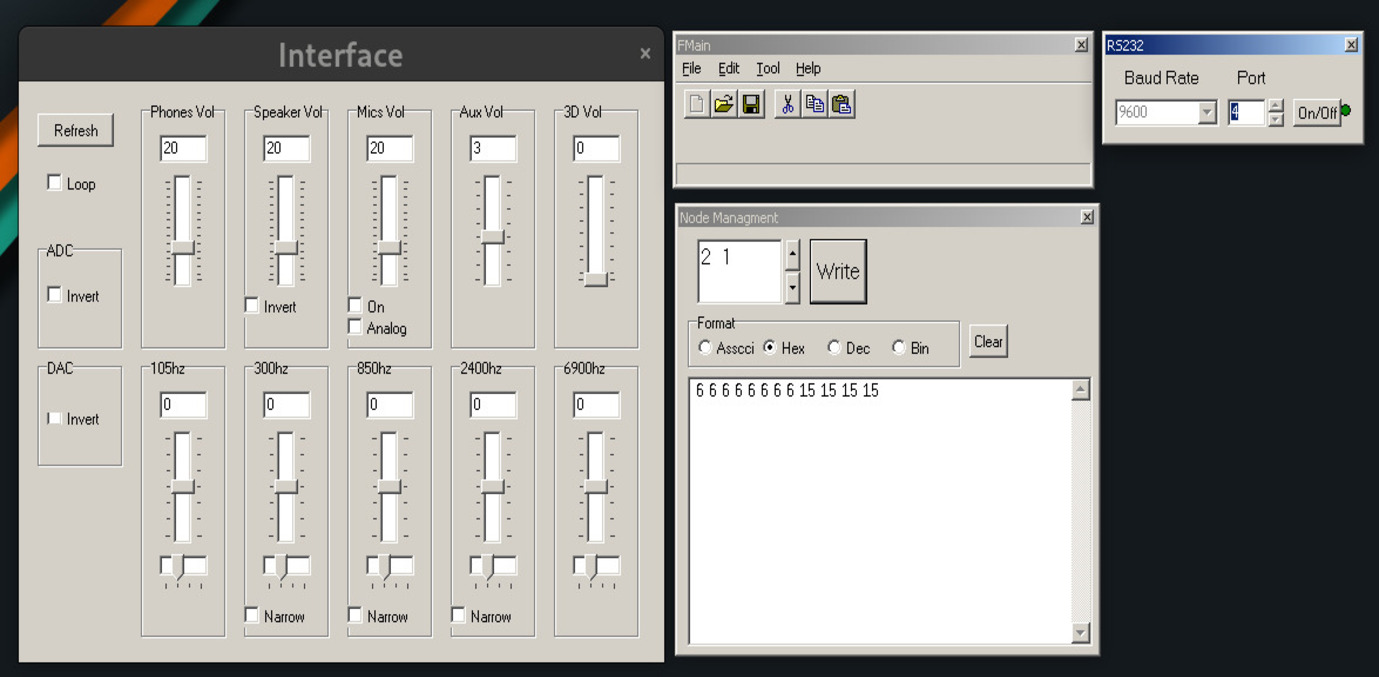
\includegraphics[width=0.3\textwidth]{vba1.jpg}
         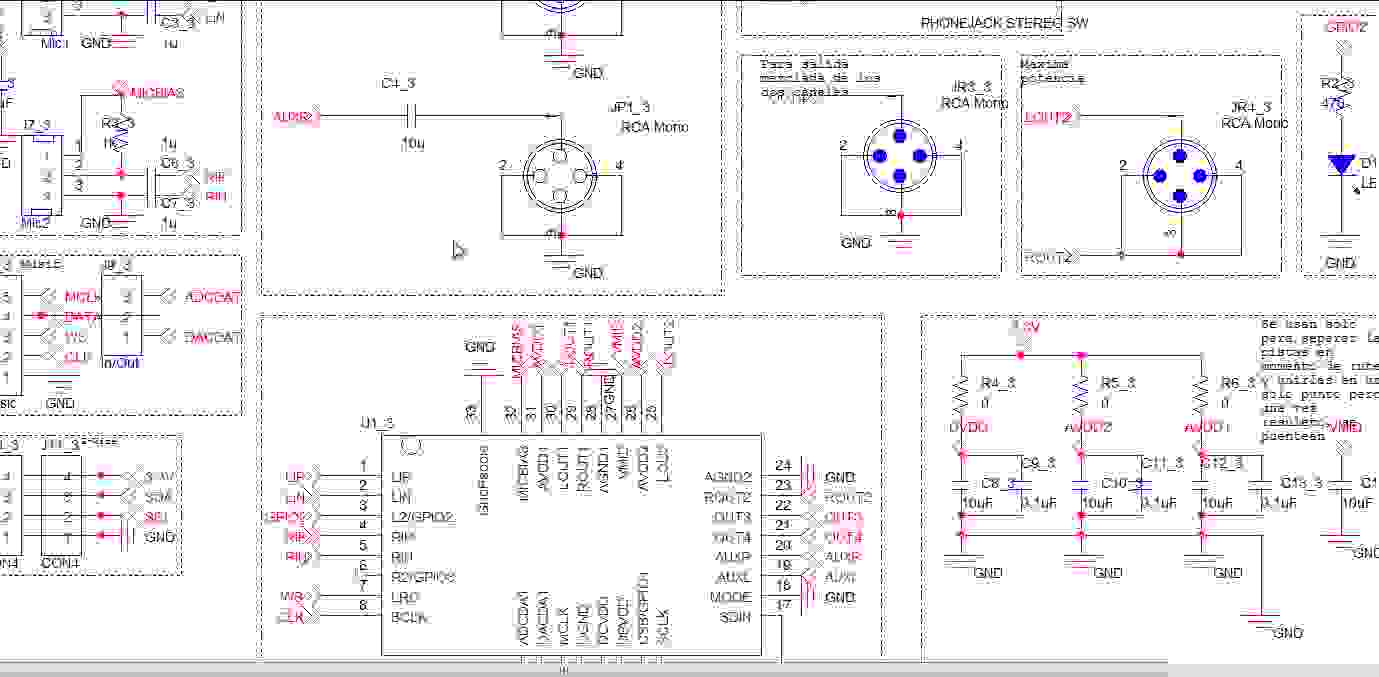
\includegraphics[width=0.3\textwidth]{vba2.jpg}
         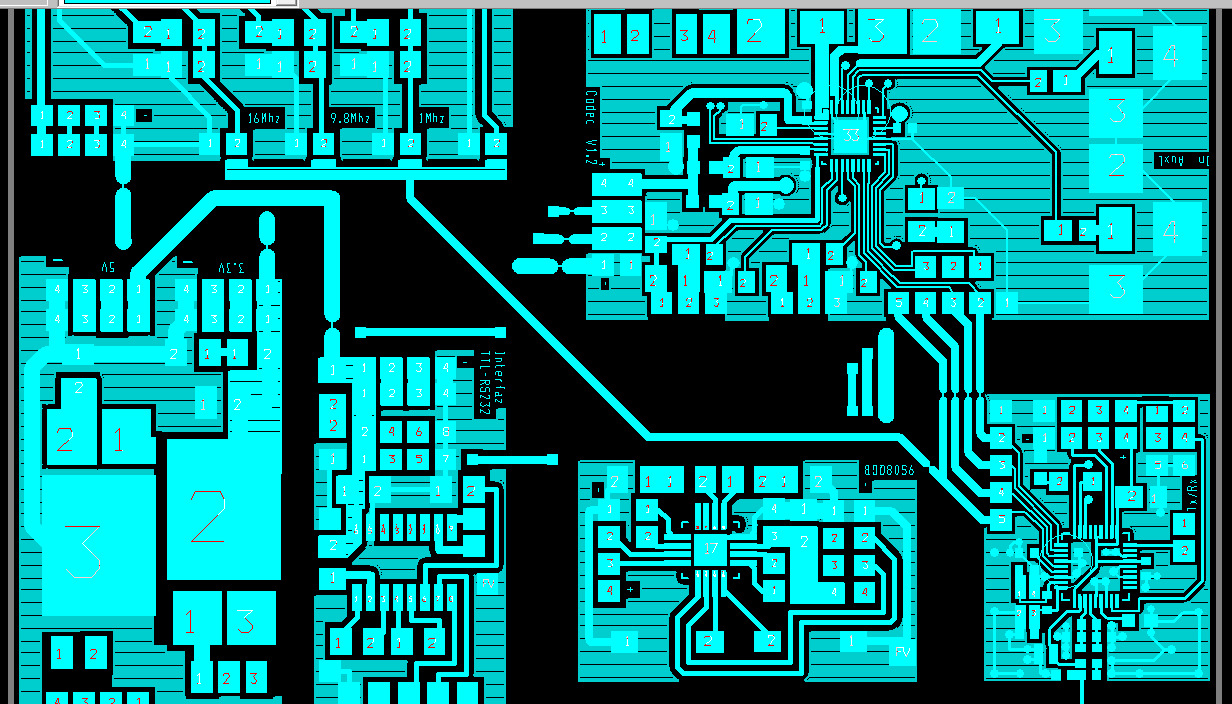
\includegraphics[width=0.3\textwidth]{vba3.jpg}
      \end{center}
        \caption{Esquemático, layout y software de calibración en Borland C++ builder para la prueba de concepto de un implante auditivo inalambrico para la empresa VBA Argentina.}
      \label{fig:vba}
   \end{figure}
